\chapter{\K{}-based Computer Interpretable Guidelines}

In \autoref{chapter:separating-concerns}, we described an
architecture for building safe and modular clinical decision support systems.
We split \CDSSs{} into three separate components:
\begin{enumerate*}[label=(\alph*)]
  \item a frontend that facilitates interaction with \HCPs{},
  \item a backend that serves as a computer-interpretable encoding of the \BPG{}, and,
  \item additional infrastructure that wires components together.
\end{enumerate*}
This, and upcoming chapters, focus on building backends for \CDSSs{}
utilizing the \emph{semantics-first} approach described in
\autoref{chapter:semantics-first-cdss}. By semantics-first, we
mean that:
\begin{enumerate*}[label=(\alph*)]
 \item the semantics of medical knowledge in the \BPG{} is
 accurately captured, and,
 \item the semantics of the language used to describe the
 \BPG{} is formally defined.
\end{enumerate*}

In \autoref{sec:generic-bpg}, we briefly described characteristics
of \BPGs{} that a \CIG{} language must accommodate.
To this end, we attempted to come up with a framework that
can accommodate expressing a large number of diverse \BPGs{}.
Thus, we broke \BPGs{} into smaller statements that we organized
into:
\begin{itemize}
  \item a workflow containing statements that are executed sequentially, and,
  \item workflows within a guideline may be executed concurrently.
\end{itemize}

In this chapter, we describe a methodology to encode real-world \BPGs{}
as $\K$ definitions. Execution in $\K{}$ is inherently concurrent---
if more than one $\K{}$ rule can apply, then $\K$ non-deterministically
chooses one. Thus, we describe a way of systematically encoding
medical knowledge in \BPGs{} as $\K$ definitions. First, in
\autoref{sec:acls}, we introduce a real world \BPG{} that will be
utilized as running-example in the rest of this chapter. Note that
we intentionally choose real-word examples, instead of small toy cases,
to highlight that our philosophy scales to work in the real-world.
Next, \autoref{sec:kacls-cdss} describes $\KACLS{}$, a $\K$-based tool
to assist \HCPs{} conform to \ACLS{} guidelines that attempts to
follow the \emph{semantics-first} approach. Specifically,
we come up with an abstract representation that captures the semantics
of the \BPG{} from \autoref{sec:acls} with enough details to
enable computer-interpretation. Finally, in \autoref{sec:kacls-backend},
we describe a way to embed said abstract representation into a concrete
$\K$ definition for execution.

\section{Advanced Cardiovascular Life Support Guidelines (\ACLS{})}\label{sec:acls}

\begin{figure}[t!]
  \centering
  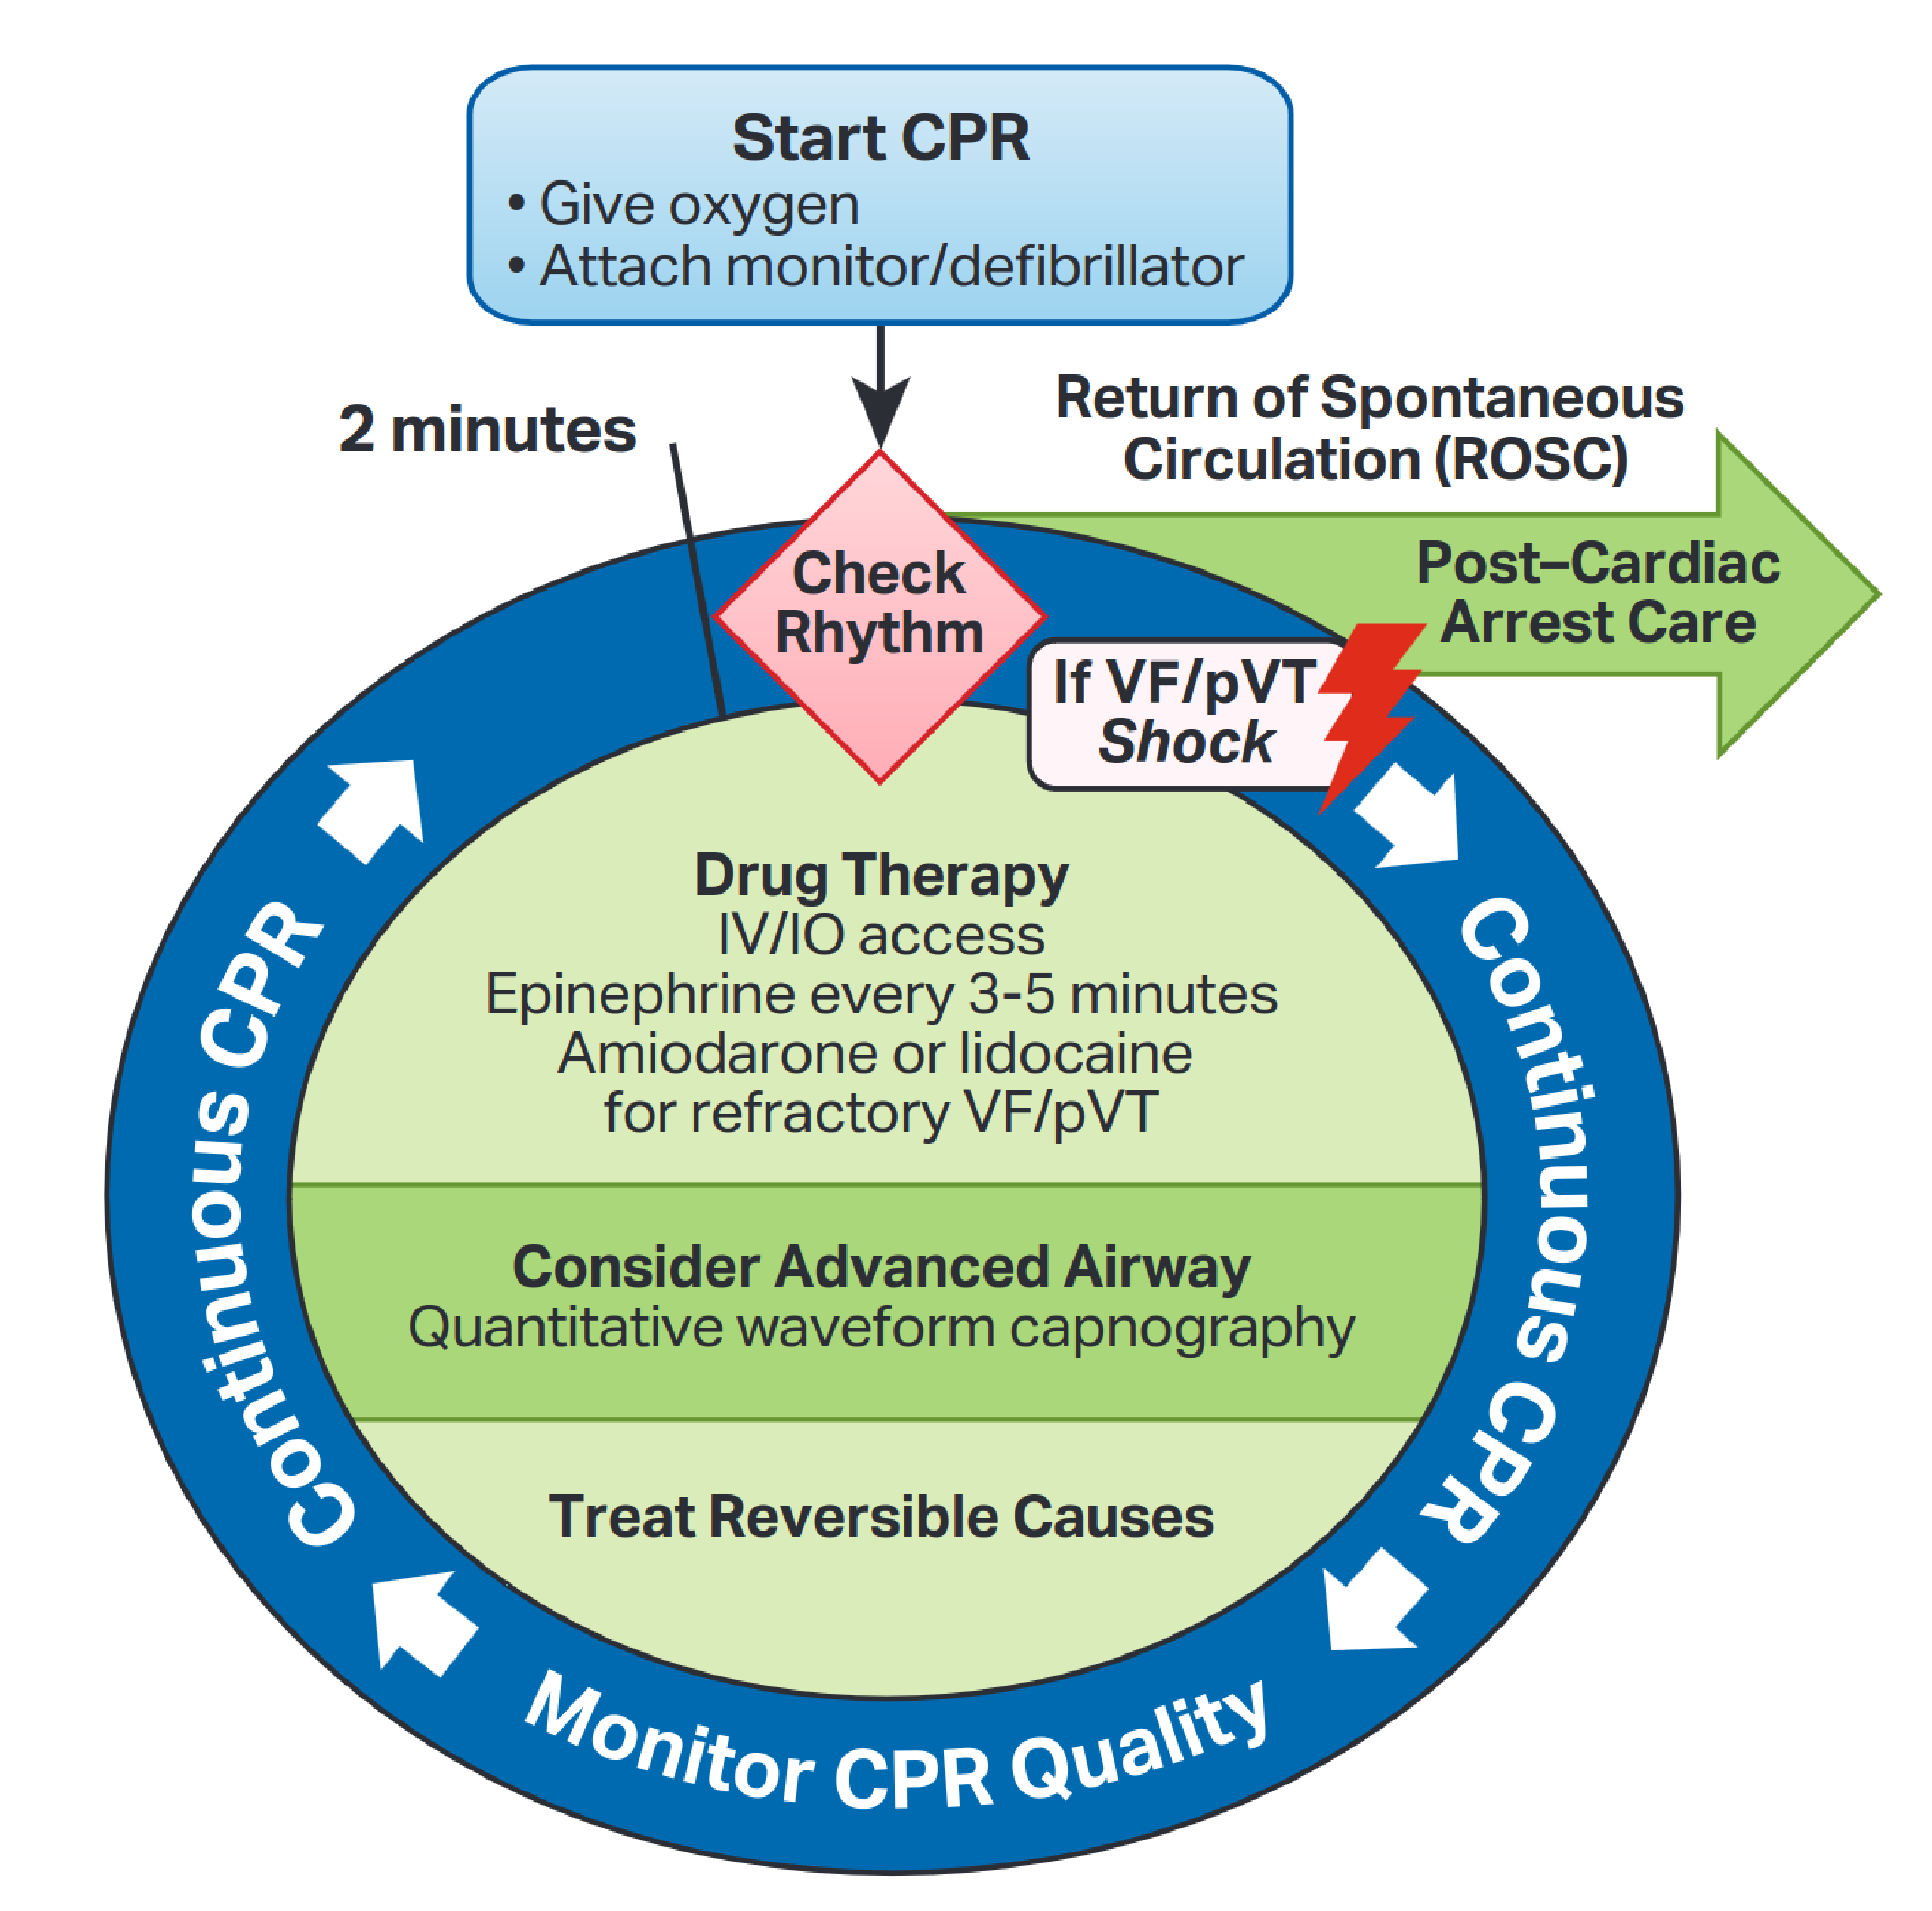
\includegraphics[width=0.6\textwidth]{acls-algorithm}
  \caption{Advanced Cardiac Life Support Guidelines}\label{fig:acls-algorithm}
\end{figure}

Advanced Cardiovascular Life Support (\ACLS{}) are a set of \BPGs{} periodically
published by the American Heart Association (\AHA{}) for management of
life-threatening cardiac conditions that will cause of have caused cardiac
arrest. The conditions that the guidelines treat range from dangerous arrhythmias, i.e.,
irregularities in heart's rhythm, to cardiac arrest.---a cardiac emergency where
the heart stop pumping \cite{ACLSWikiEntry}.
The guidelines, according to the AHA{}, \say{are based on the most current
and comprehensive review of resuscitation science, systems, protocols, and
education} \cite{ACLSUrl}.

\autoref{fig:acls-algorithm} shows the \AHA{}'s guidelines for advanced
life support (\ALS{}) for managing cardiac arrest in adults \cite{ACLSGuidelineUrl}.
\AHA{} publishes guidelines
for basic life support (\BLS{}), and pediatric counterparts of both. While
\BLS{} is meant for a first responder to provide treatment with
limited resources, such as an automatic emergency defibrillator (\AED{}),
\ACLS{} is supposed to be followed by teams of
trained professionals with advanced equipment for airway management,
drug delivery, etc.

\subsubsection{Why build \CDSSs{} for \ACLS{}?}

Cardiac arrest treatment is extremely time-critical, and outcomes
become significantly worse with every passing minute. This
gathering relevant data about the patient infeasible. Moreover, as
the seriousness of the condition necessitates multiple, simultaneous treatments
to be administered rapidly, intervention is usually executed following
standardized \ACLS{} algorithms \cite{ACLSWikiEntry}.

Prompt \ACLS{} guidelines-conformant treatment has been
shown to improve patient outcomes \cite{HonarmandResuscitation18}.
Moreover, deviations from the guidelines in in-hospital cases has been
associated with decreased rates of return of spontaneous circulation (\ROSC{}),
survival to discharge, and survival to discharge with favorable neurological
outcomes \cite{CrowleyResuscitation20}. Studies have also found that
inadequate \ACLS{} training can lead to poor retention, resulting
in reduced \ACLS{} conformance \cite{KiddJCN07}. Thus,
a \CDSS{} that can provide situation-specific guidance about
the next steps, especially in cases where \HCP{} training might be inadequate,
can potentially improve compliance, and consequently outcomes.

\subsubsection{A Brief Overview of Advance Life Support Guidelines for Cardiac Arrest:}

As we aren't concerned with intricacies of medical knowledge in the guideline,
we present a brief and simplified description of the guideline-prescribed treatment.
As \ALS{} is supposed to be performed in settings where necessary equipment is
available, a electrocardiogram (EKG) machine is utilized to
monitor the patient's cardiac rhythm. Certain cardiac arrhythmias, characterized
by cardiac rhythms referred to as \emph{shockable}, must be treated
by delivering a therapeutic electric shock
\cite{DefibrillationWikiEntry}. As shown in \autoref{fig:acls-algorithm},
treatment has several parallel workflows such as:
\begin{itemize}
  \item Periodic monitoring of the cardiac rhythm, and in case of a
    \emph{shockable} rhythm, using a defibrillator.
  \item Continuous cardiopulmonary resuscitation (\CPR{}).
  \item Administration of vital drugs such as
    epinephrine every few minutes.
\end{itemize}
As \autoref{fig:acls-algorithm} suggests, these workflows have to be
performed rapidly and periodically. As the duration of the intervention
is typically a few minutes, making optimal use of available time is critical to
outcomes.

\section{The \KACLS{} System}\label{sec:kacls-cdss}

\begin{figure}[t!]
  \centering
  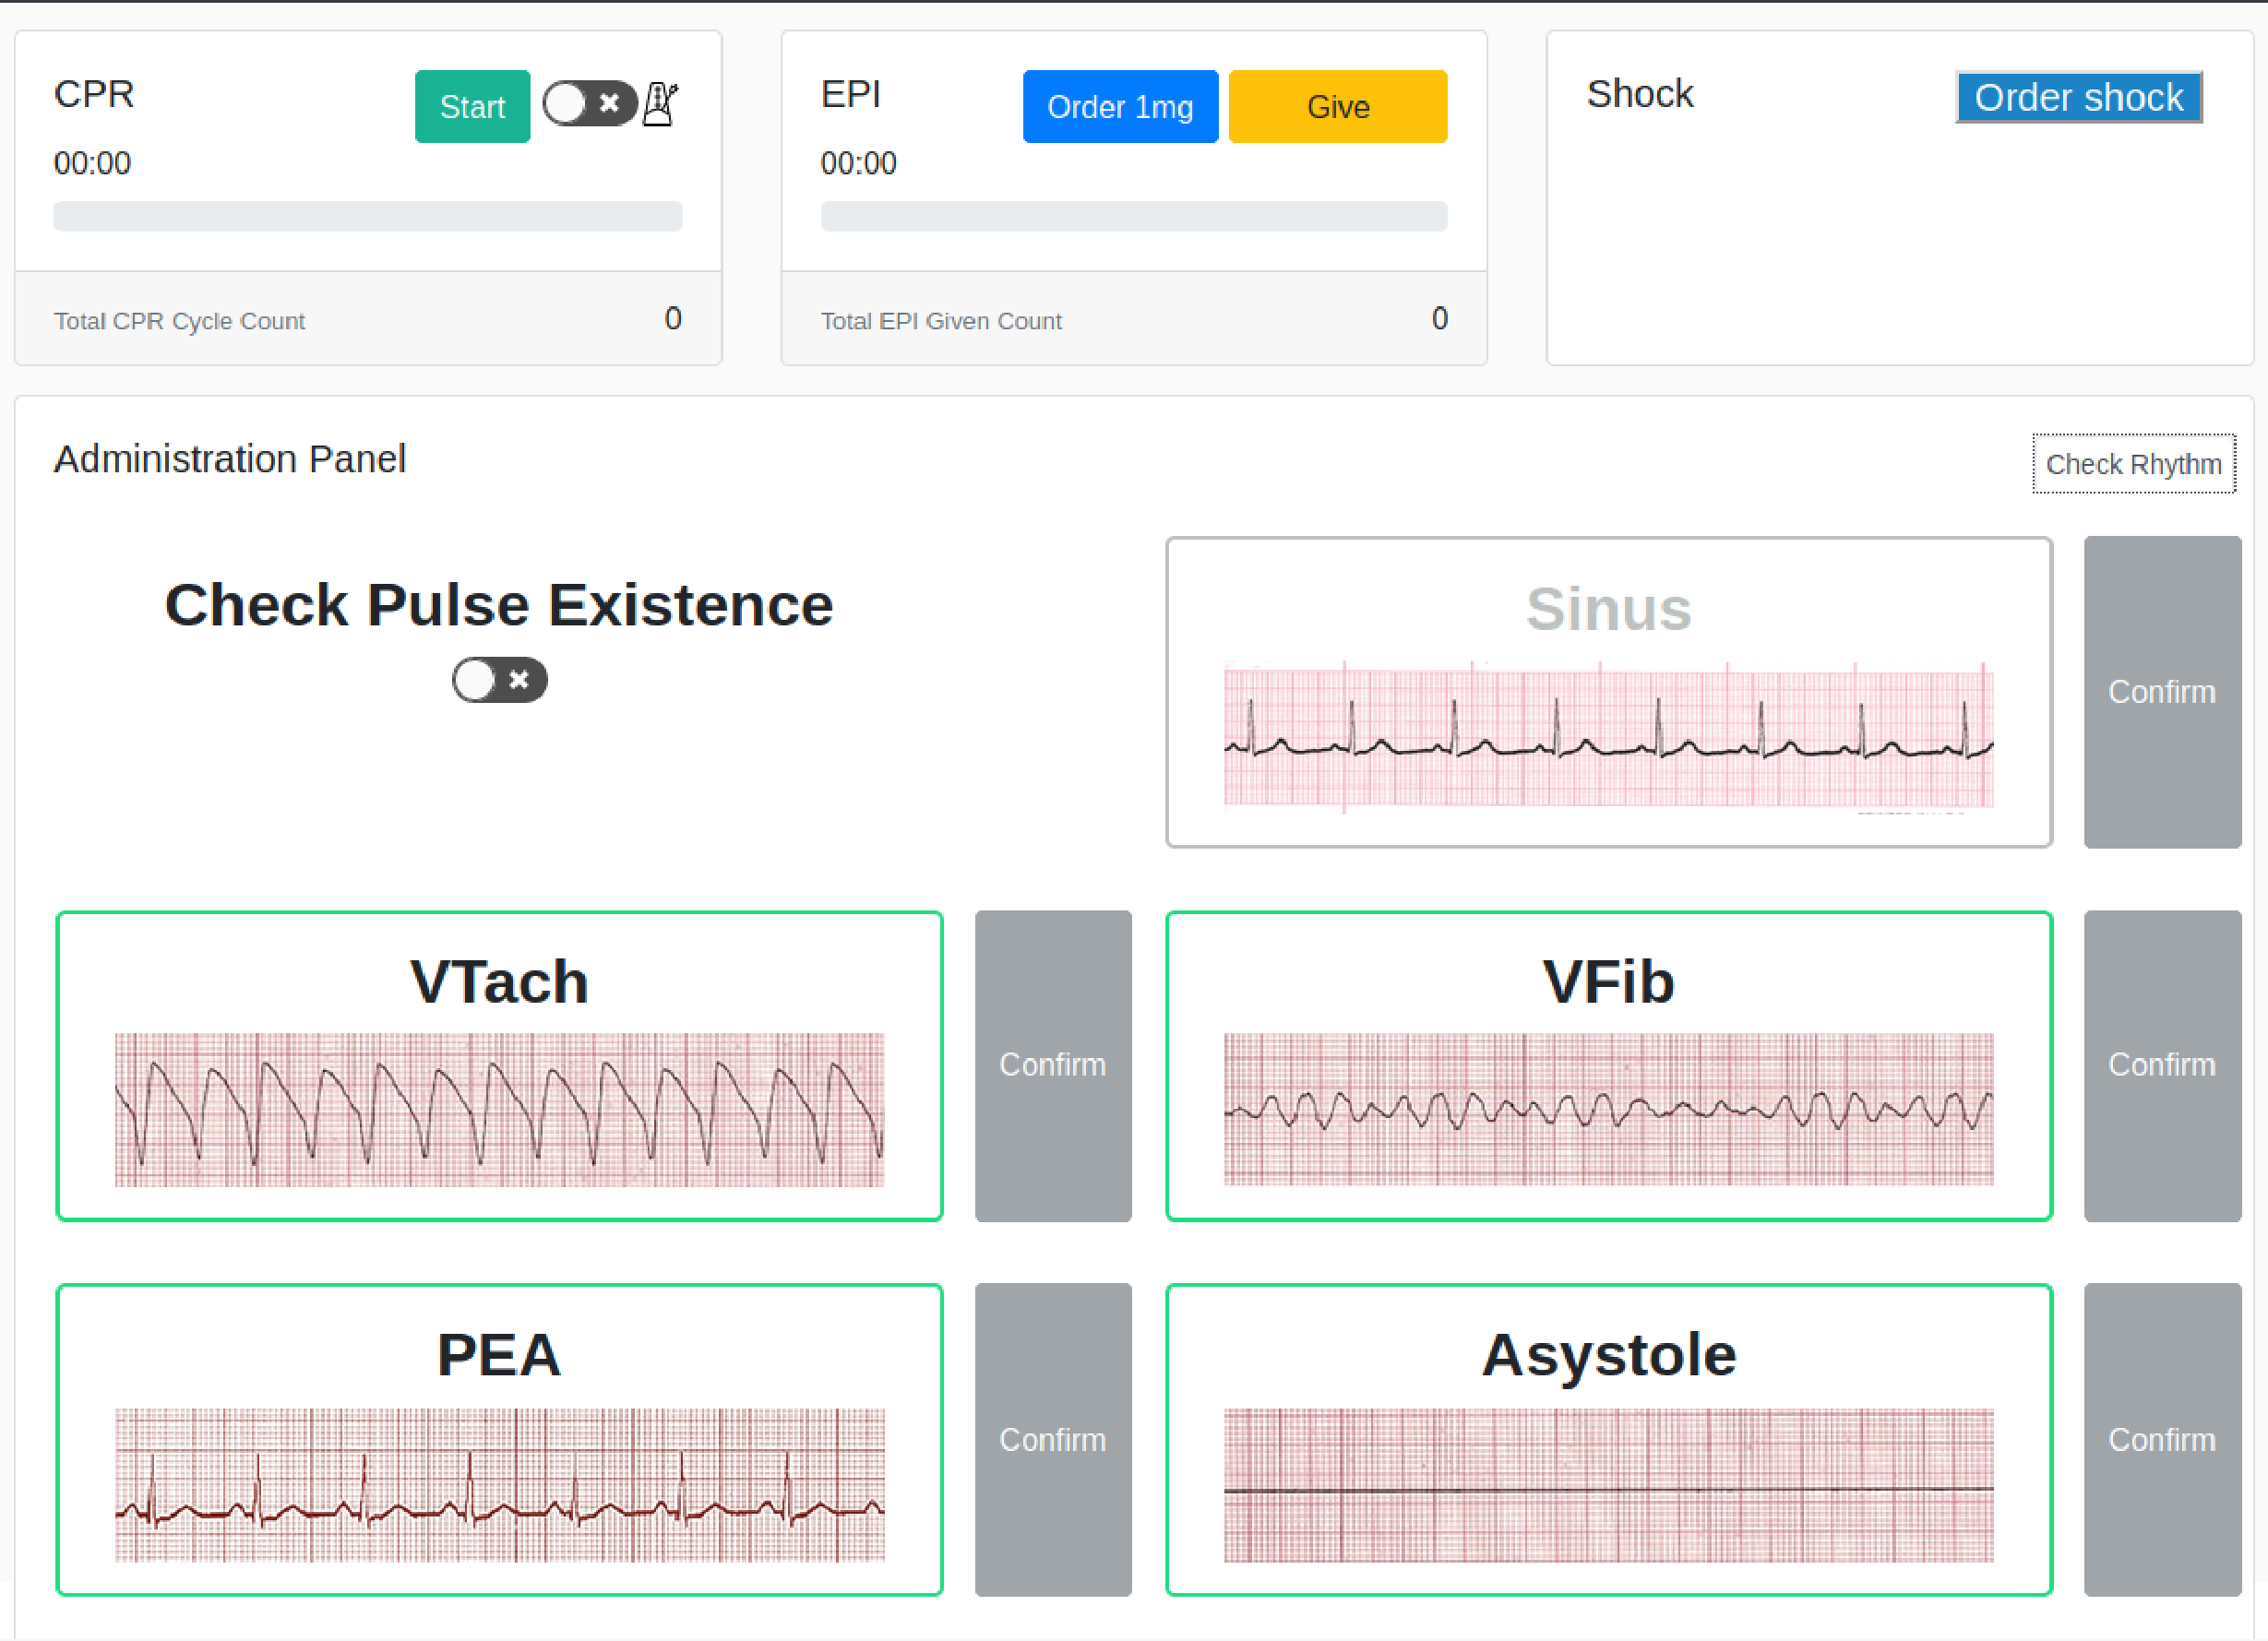
\includegraphics[width=0.85\textwidth]{acls-tool}
  \caption{Snapshot of \KACLS{}}\label{fig:kacls-snapshot}
\end{figure}

\autoref{fig:kacls-snapshot} shows a snapshot of our \CDSS{} for
enabling compliance to the advanced life support guidelines described in
\autoref{sec:acls}. Advanced life support is supposed to be performed by
a team of \HCPs{}, that take on roles such as a leader, \CPR{}-provider,
airway/respiratory specialist, Intravenous access (IV) and drug administration
specialist, pharmacist, defibrillator attendant and members that serve as
backups \cite{ACLSWikiEntry}. The leader is responsible for coordinating
treatment, our tool render support through a handheld tablet held by the leader.
\autoref{fig:kacls-snapshot} show a snapshot of said tablet's main screen.
Decision support, in the form of time-sensitive reminders, warnings when
procedures are stopped prematurely, or exceed stipulated limitations, and
confirmations regarding the patient rhythm's are provided on the screen
through popups and progress bars. For example, when the leader instructs
the team to start CPR, and presses the \say{Start} button under the \say{CPR}
section of the screen. A timer displays the duration and appropriate warnings
about prematurely stopping CPR, or exceeding the time for a \CPR{} cycle are
displayed.

\subsection{Capturing Execution-specific Details}\label{sec:execution-specific-details}

A computer-interpretable version of a guidelines, unlike its
textual counterpart, may require specification of additional details
for execution. Such details can often be gathered from context in case
of textual guidelines, or may be unintentionally missing. This was also
discussed in context of related approaches in \autoref{chapter:related-work},
especially in \autoref{sec:kiv-verification}.

As discussed in \autoref{sec:generic-bpg}, \BPGs{} can be notionally
represented using a collection of workflows. Each workflow has steps
executed sequentially, but may be concurrently executed with steps from
other workflows. Consider the \ACLS{} guidelines discussed in
\autoref{sec:acls}. Several procedures, such as administering drugs,
and performing \CPR{} occur concurrently, where each procedure has
a set of tasks that need to be performed sequentially.
There may also be some implicit order across workflows, but we
address that in later chapters.

\subsubsection{Modeling \BPGs{} as State Machines}

In this work, we choose to express medical logic using
concurrently executing finite state machines that communicate
with implicit queues for inter-machine communication. Communicating
state machines (\CSMs{}) is a well-understood model of concurrency
\cite{BrandJACM83}, and is well-suited  representing medical guidelines in a
computer-interpretable format that is also \HCP{}-friendly.
We shall discuss the motivations behind using \CSMs{} in upcoming
chapters. For now, it suffices to describe how our choice addresses
issues mentioned in \autoref{sec:execution-specific-details}.
Given a guideline represented as a collection of workflows, we
describe each workflow via a state machine. The fact that
\CSMs{} can execute concurrently conveniently captures the
inherent concurrency in workflows.

\subsubsection{\ACLS{} Workflows As State Machines}

\autoref{fig:machine-defs} shows \ACLS{} workflows formalized
as state machines. \autoref{fig:cpr-machine} captures the
guideline specified procedure for administering \CPR{}.

In \autoref{sec:modular-cdss-architecture}, we described
conceptual components of \CDSSs{}, and argued in favor
of developing \CDSSs{} using independently developed and maintained codebases
aligned with these components. The \KACLS{} system follows
this philosophy, and has:
\begin{enumerate*}[label=(\roman*)]
  \item a simple \emph{frontend} written in ReactJS that handles
    user interaction, and,
  \item a $\K$-based HTTP server that encodes the \ACLS{} guideline
    and interacts with the frontend.
\end{enumerate*}
The use of a Javascript based simple frontend allows our application
to run on any modern web-browser. As shown in figure \ref{fig:acls-tool},
our frontend consists of forms and buttons that correspond to procedures
in the algorithm in figure \ref{fig:acls-algorithm}. For example, the
\say{Start} button in the CPR box results in a two minute timer corresponding
to the \say{2 minute continuous CPR} procedure in the informal description.
The frontend is simple and doesn't contain any guideline conformance related
logic. Interaction with the frontend simply results in dispatch of
\textit{events} to the backend. For example, when the \say{Start} button is pressed, a
\say{StartCpr} event is sent to the backend.






\begin{figure}[tb]
\centering
\begin{subfigure}{\textwidth}
  \centering
  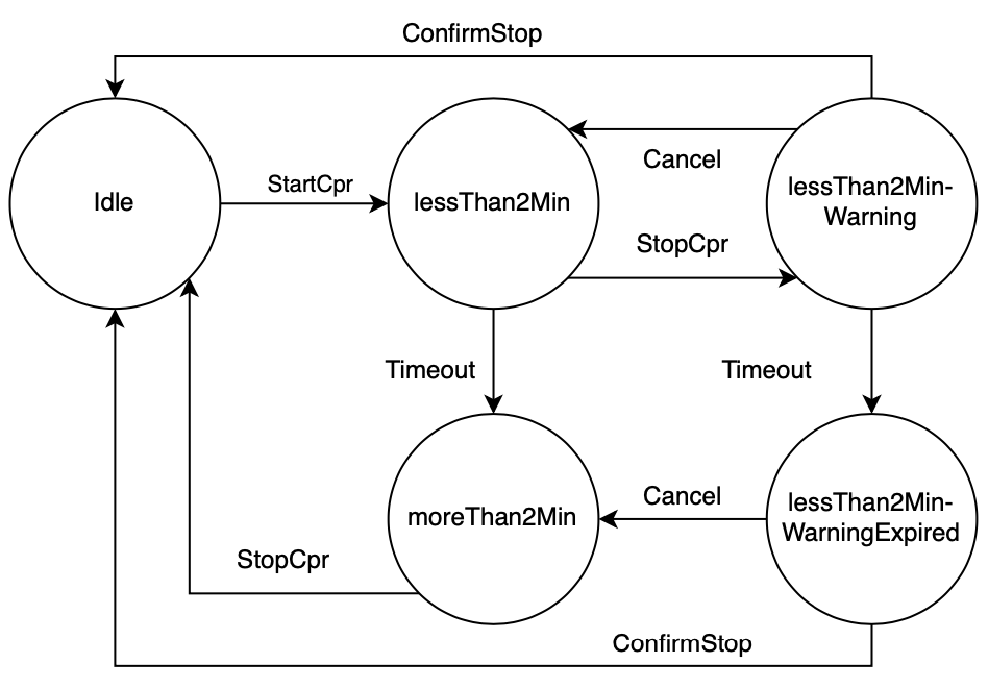
\includegraphics[width=0.65\linewidth]{cpr-machine}
  \caption{CPR Machine}
  \label{fig:cpr-machine}
\end{subfigure}%
\hfill\newline\hfill\newline\hfill
\begin{subfigure}{\textwidth}
  \centering
  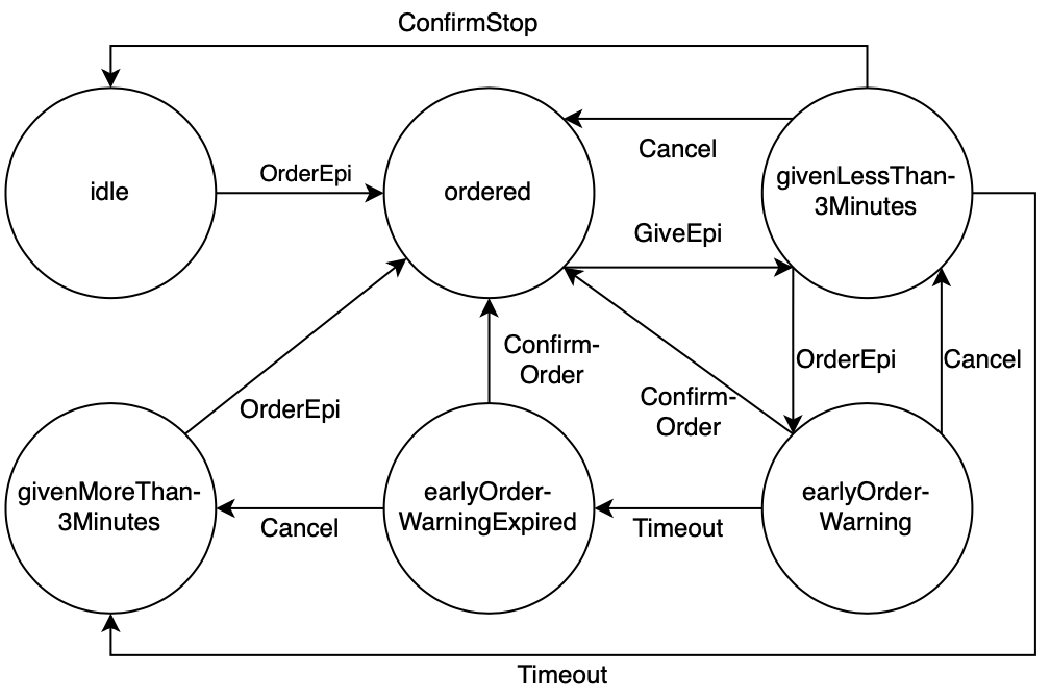
\includegraphics[width=0.65\linewidth]{epi-machine}
  \caption{Epinephrine Machine}
  \label{fig:epi-machine}
\end{subfigure}
\caption{Formal Machine Definitions}
\label{fig:machine-defs}
\end{figure}

\subsection{$\KACLS$ backend}\label{sec:kacls-backend}




